%!TEX root=../document.tex

\section{Ergebnisse}
\label{sec:Ergebnisse}

Hier werden sie meine Ergebnisse zu den vorher aufgezählten Aufgabestellungen



\subsection{Aufgabe 1}
In der zurverfügung gestellten VM Ubuntu habe ich mich in den lokalen LADP Server als admin eingelogged und dann 5 User und 2 Gruppen erstellt
Hier sieht man die Gruppen(group.service2-4) und die User(user1-5) die ich erstellt habe.

\begin{figure}[!h]
	\begin{center}
		\includegraphics[width=0.3\linewidth]{images/aufgabe_1.png}
		\caption{User und Groups Liste \cite{tanenbaum2007verteilte}}
		\label{broker}
	\end{center}
\end{figure}​

Um dies zu schaffen habe ich aus den vorgegebenen Templates Poxis Group für die Gruppen und User Account für die User benutzt.

\clearpage
\subsection{Aufgabe 2}
\clearpage

\subsection{Aufgabe 3}
\subsubsection{Beispiel}
\begin{figure}[!h]
	\begin{center}
		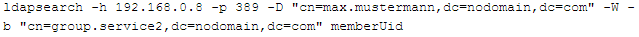
\includegraphics[width=1\linewidth]{images/example.png}
		\caption{Beispiel zur Suche \cite{tanenbaum2007verteilte}}
		\label{broker}
	\end{center}
\end{figure}
-h.....Die adresse des Servers\\
-p.....Die Port Nummer\\
-D.....Als wer man sich anmelden will\\
-W....Das ich nach dem Passwort abgefragt werde(sonst muss ich es als Parameter eingeben)\\
-b.....Nach was ich suche\\
\subsubsection{erste Suche}
Wir sollen mi dem Terminal auf den lokalen LDAP-Server zugreifen und 3 Suchanfragen starten und dokumentieren. 

\begin{figure}[!h]
	\begin{center}
		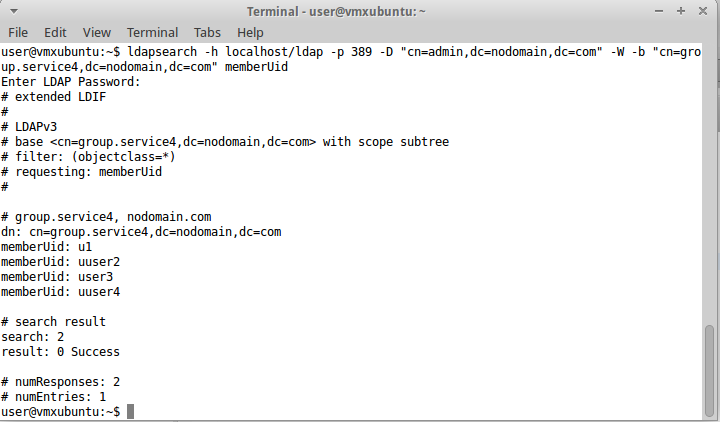
\includegraphics[width=0.8\linewidth]{images/1stSearch.png}
		\caption{erste Suche \cite{tanenbaum2007verteilte}}
		\label{broker}
	\end{center}
\end{figure}
Hier sieht man das ich mich als admin eingelogged habe und dann die memberUid von allen Usern aus der Gruppe group.service4 rausgesucht hab.\\
\subsubsection{zweite Suche}

\begin{figure}[!h]
	\begin{center}
		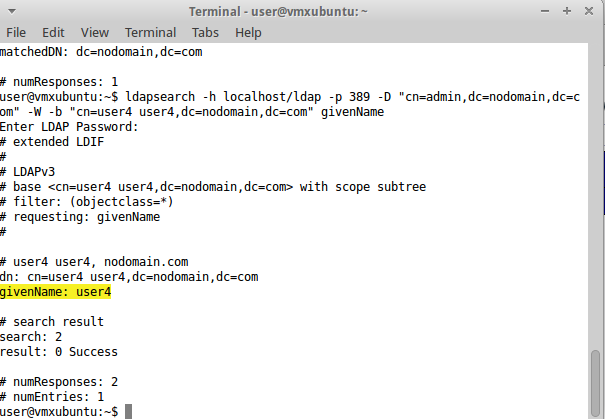
\includegraphics[width=0.8\linewidth]{images/2ndSearch.png}
		\caption{zweite Suche \cite{tanenbaum2007verteilte}}
		\label{broker}
	\end{center}
\end{figure}
Hier sieht man das ich mich wieder als admin eingelogged hab aber dieses mal nach dem givenName eines bestimmten Users(user4) gesucht hab.
\clearpage	

\subsubsection{dritte Suche}

\begin{figure}[!h]
	\begin{center}
		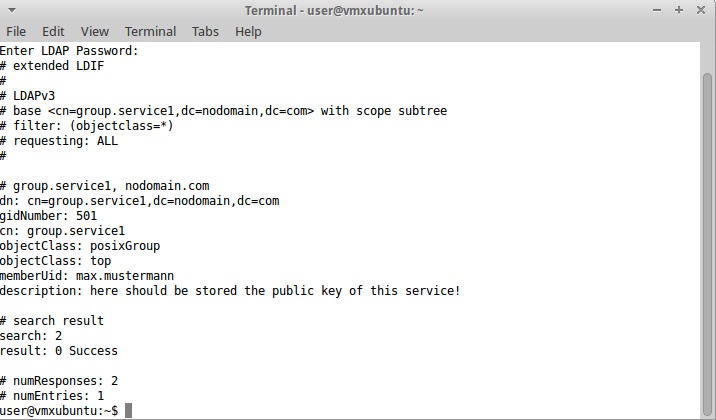
\includegraphics[width=0.8\linewidth]{images/3rdSearch.png}
		\caption{dritte Suche \cite{tanenbaum2007verteilte}}
		\label{broker}
	\end{center}
\end{figure}
hier habe ich nach der Gruppe group.service1 gesucht und es wurde dann alle information über die Gruppe zurückgegeben.

%%%%%%%%%%%%%%%%%%%%%%%%%%%%%%%%%%%%%%%%%%%%%%%%%%%%%%%%%%%%%%


%%%%%%%%%%%%%%%%%%%%%%%%%%%%%%%%%%%%%%%%%%%%%%%%%%%%%%%%%%%%%%%%
